% !TEX root = ../main.tex
%
\chapter{Time Series Feature Extraction}
\label{sec:feature-extraction}
\vspace*{-15mm}
\hfill{\fontfamily{phv}\normalsize\emph{Paul Fährmann and Sanjay Gupta}}

\cleanchapterquote{The best feature is less features.}{Kevin Systrom}{(Computer programmer and entrepreneur)}

% Motivation Section start.
\section{Motivation}
\vspace*{-15mm}
\hfill{\fontfamily{phv}\normalsize\emph{Sanjay Gupta}}
\\\\
In recent years, the development of Industry 4.0, the Internet of Things (IoT) has led to the availability of several types of sensors on the market at a low price, which drives the industry to use the sensor in a machine that generates an enormous amount of data in the form of time series. This data helps the engineer or scientist to analyze and to maintain the health of the machine in order to avoid unwanted failures in the near future. One of the preliminary steps in ML pipelines is the process of extracting time series data. We can not directly use raw data because it is noisy. So we extract features to different domains, i.e. time domain and frequency domain, to remove noise and unwanted data, and to extract a set of useful features that will help to understand the behavior of the system. The purpose of the feature vector set is to characterize the data of the time series. Finally, this vector of features is fed to several ML classifiers or method to predict the health status, health index, and lifespan of the system.
% Motivation Section end.

% Formal Definition Setion start.
\section{Formal Definition}
\label{sec:feature-extraction:formal-definition}
\vspace*{-15mm}
\hfill{\fontfamily{phv}\normalsize\emph{Paul Fährmann}}
\\\\
For time series feature extraction we want to condense the most important and characterizing information about a time series into a fixed length representation. That is useful for machine learning approaches that cannot work with inputs of various lengths (e.g. SVM). The time series consists of data from different sensors and thus we can combine features extracted from these different sensor data into one feature representation.
For a specific time series we will define our feature representation as a real-valued vector of fixed length $d \in \mathbb{N}$.
\begin{equation}
z = (z_1, \dots, z_k) \in \mathbb{R}^d
\end{equation}
The problem of feature extraction then results in creating a mapping from a time series as defined in Subsection~\ref{sec:intro:time-series-definition} to our feature representation vector.
For this a feature extraction method $g$ maps an instance $x\in\mathcal{X}$ to our feature representation $z\in\mathbb{R}^d$.
\begin{equation}
\label{eq:fe_no_label}
g: \mathcal{X} \longrightarrow \mathbb{R}^d
\end{equation}
That means the whole time series gets represented in one single vector that contains the most important information of that time series.\\
Some feature extraction methods need class labels in order to work. Hence, we need to differentiate between supervised and unsupervised feature extraction.
For the unsupervised case, the definition in Equation~\ref{eq:fe_no_label} works as we don't include class labels in our mapping. For the supervised case we need to include class labels as follows:
\begin{equation}
\begin{split}
g: \quad \mathcal{X}  \times\mathcal{Y} &\longrightarrow \mathbb{R}^d \\
\end{split}
\end{equation}
We annotate the labels with $y\in \mathcal{Y}$ where $\mathcal{Y}$ consists of the class labels used for a specific time series in a machine learning setting. $x\in\mathcal{X}$ defines an instance of a time series and $z\in\mathbb{R}^d$ is the feature representation vector.
% Formal Definition Setion end.

% Approaches Setion start.
\section{Approaches}
\vspace*{-15mm}
\hfill{\fontfamily{phv}\normalsize\emph{Sanjay Gupta \& Paul Fährmann}}
\label{sec:feature-extraction:approaches}
\\\\
As mentioned in the data-driven model, temperature, vibration, dynamic force, electrical current, and rotational speed signal are used for machine health monitoring. From all these parameters, the vibration signal is the most used condition monitoring data for fault diagnosis, commonly in rotating machines. The system failure is initially identified from the vibration data of the sensors. As a result, a vibration signal can be used to diagnose faults because it represents the dynamic features of the machine. The vibration signal collected by the sensors is often noisy, and therefore cannot be used directly for an effective fault diagnostic. Feature extraction techniques can be used to minimize the noise, which will help to detect a fault in the signal. Fault diagnosis is divided into four parts as follows: data acquisition, feature extraction, fault detection, and identification as shown in Figure \ref{fig:OverviewFaultDiagnosis}.
\begin{figure}[h]
	\centering
	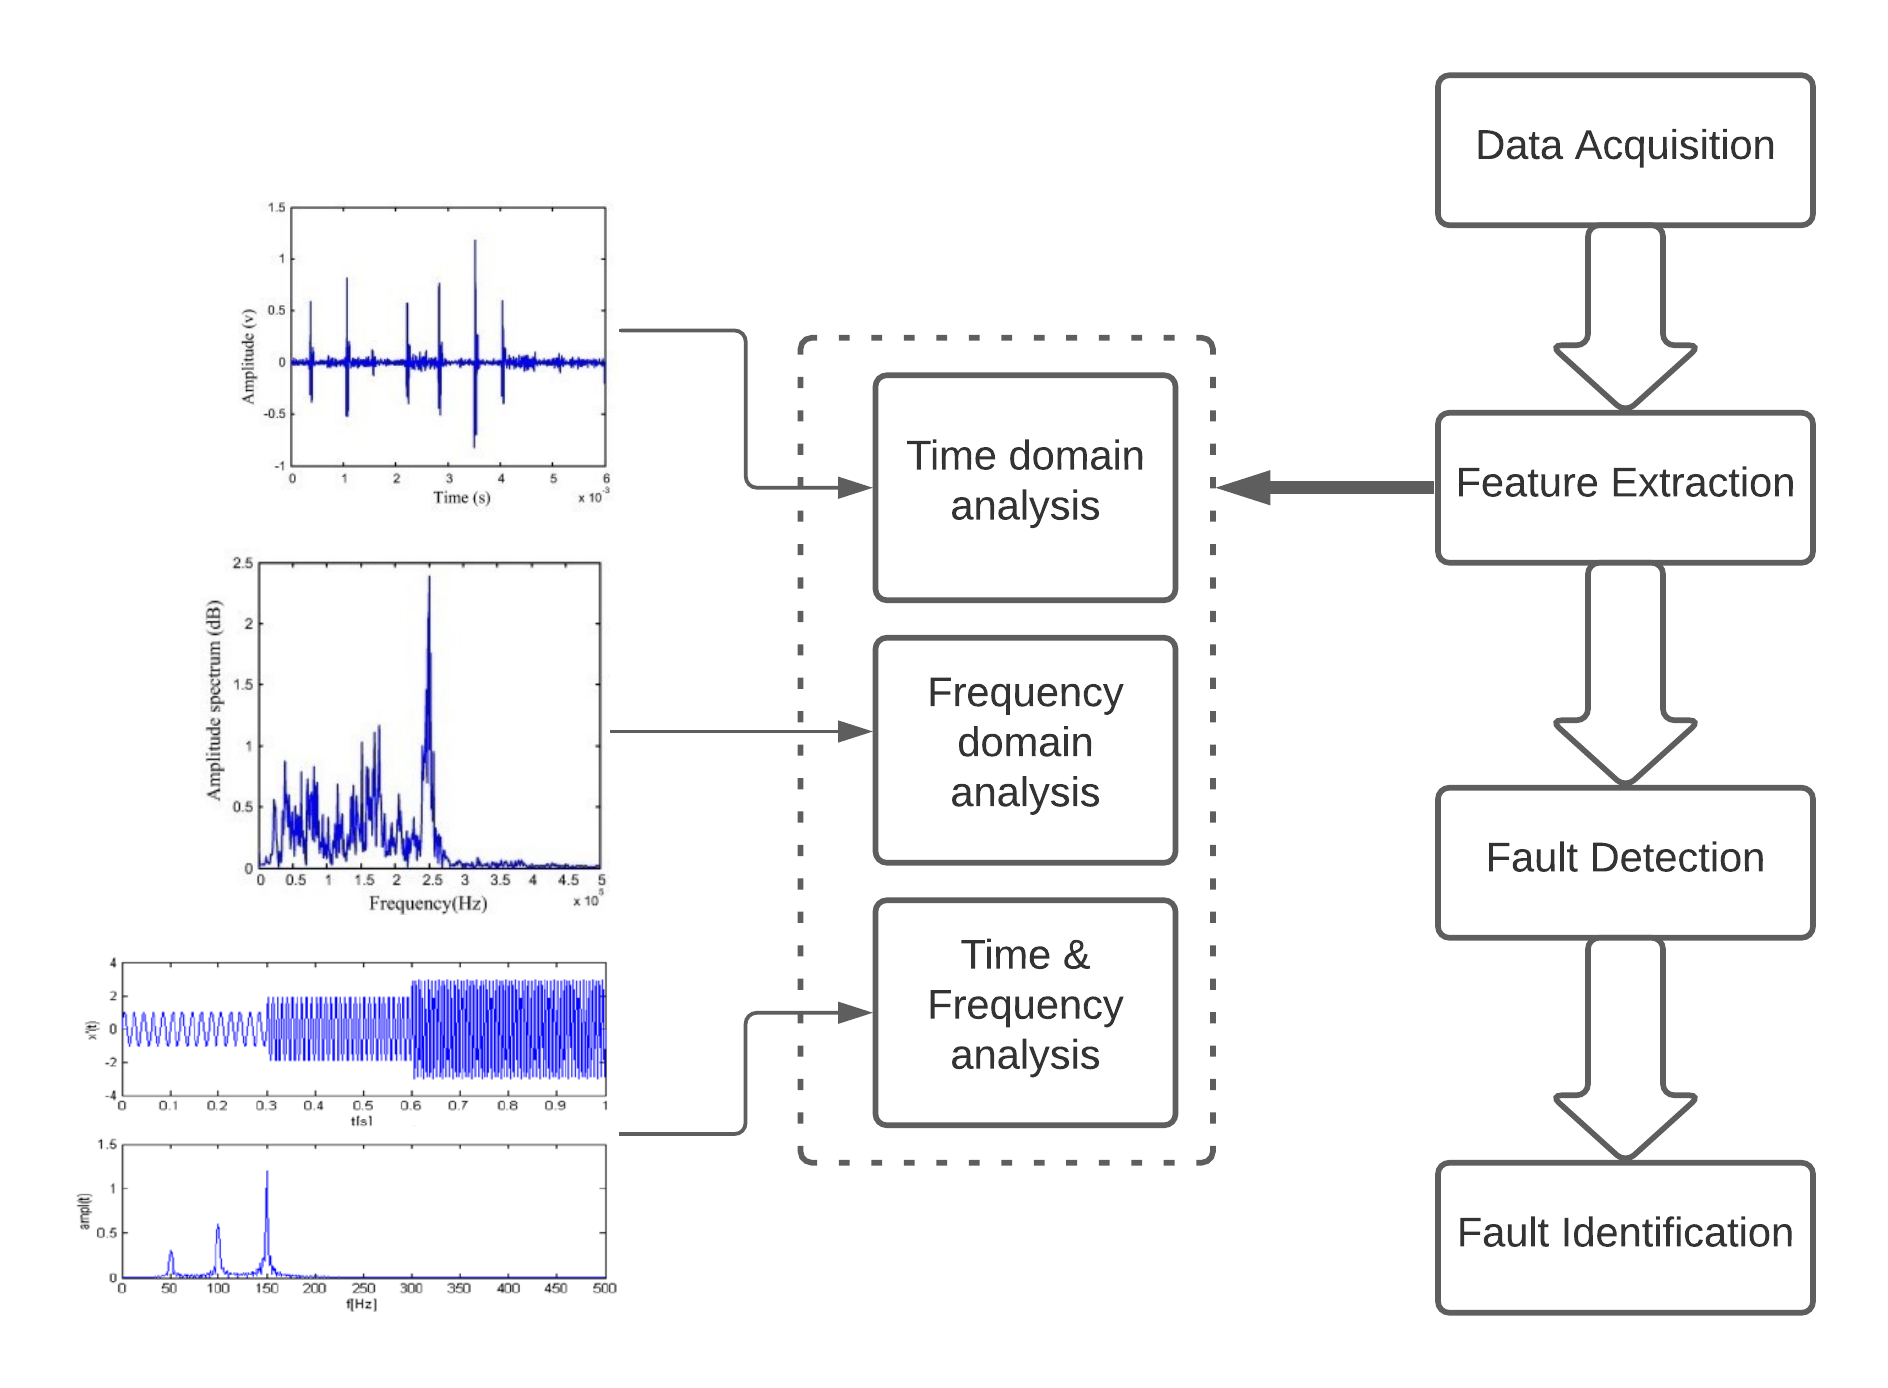
\includegraphics[width=\textwidth]{gfx/Overview of fault diagnosis based on vibration signals.png}
	\captionsetup{justification=centering}
	\caption{Overview of fault diagnosis based on vibration signals.}
	\label{fig:OverviewFaultDiagnosis}
\end{figure}
The different approaches of feature extraction are categorized into time domain, frequency domain, and time \& frequency domain methods and also include some windowing techniques that can be used in some of the methods. Whenever a method can only be used on the data of a singular sensor instead of the time series itself, we assume that the generated features we want to extract of different sensors are concatenated in one feature vector for the whole time series instance $x \in \mathcal{X}$.

\subsection{Time Domain}
\vspace*{-15mm}
\hfill{\fontfamily{phv}\normalsize\emph{Sanjay Gupta}}
\label{sec:feature-extraction:approaches:time-domain}
\\\\
The amount of vibration signals generated by the machine usually include statistical or mathematical (e.g. amplitude, acceleration, displacement, and velocity) data related to machine health.

\subsubsection*{Basic mathematical features}
Table \ref{table:BasicMathematicalFeatures} shows a list of time-domain features that are commonly used for PdM \cite{DBLP:phd/dnb/Kimotho16}. These features can be very effective in the detection of bearing failures, imbalances, mechanical loss, electrical failure of the motor, and gearbox failures. The most basic method for measuring time-domain faults is to use the value of the Root Mean Square (RMS). The RMS value and Crest factor are used to diagnose gears and bearings failures \cite{TANDON1999469}.
\begin{table}[ht]
	\centering
	\begin{tabular}{|p{3cm}|p{3cm}|p{6cm}|}
		\hline
		\vspace{-1mm} \textbf{Feature} & \vspace{-1mm} \textbf{Formula} & \vspace{-1mm} \textbf{Description} \\[3ex]
		\hline

		\vspace{-1mm} RMS Value & \vspace{-1mm} \begin{math} \sqrt{\frac{1}{n}\sum_{i=1}^{n} s_{i}^{2} } \end{math} & \vspace{-1mm} Measure the power contained in the signal. \\[3ex]
		\hline

		\vspace{-1mm} Variance & \vspace{-1mm} \begin{math} \frac{1}{n} \sum_{i=1}^{n}(s_{i}-\bar{s})^2 \end{math} & \vspace{-1mm}  Measure the variability in the signal. \\[3ex]
		\hline
		
		\vspace{-1mm} Skewness & \vspace{-1mm} \begin{math} \frac{\sum_{i=1}^{n}(s_{i}-\bar{s})^3}{(n-1)\sigma^3} \end{math} & \vspace{-1mm} Measure the asymmetry of the data around the mean. \\[3ex]
		\hline
		
		\vspace{-1mm} Entropy & \vspace{-1mm} \begin{math} - \sum_{i=1}^{n} s_{i} \log_{2}{(s_{i})} \end{math} & \vspace{-1mm} Measure the structure and complexity of time series. \\[3ex]
		\hline
		
		\vspace{-1mm} Kurtosis & \vspace{-1mm} \begin{math} \frac{1}{n} \sum_{i=1}^{n} (\frac{s_{i}-\mu}{\sigma})^4	\end{math} & \vspace{-1mm} Measure the relative peakedness or flatness of a distribution. \\[3ex]
		\hline
		
		\vspace{-1mm} Peak value & \vspace{-1mm} \begin{math} \max(|s_{i}|) \end{math} & \vspace{-1mm} Measure maximum amplitude at some time. \\[3ex]
		\hline
		
		\vspace{-1mm} Peak to peak & \vspace{-1mm} \begin{math} \max(s_{i}) - \min(s_{i}) \end{math} & \vspace{-1mm} Measure the maximum excursion of the signal. \\[3ex]
		\hline
		
		\vspace{-1mm} Crest factor & \vspace{-1mm} \begin{math} \frac{Peak}{RMS} \end{math} & \vspace{-1mm} Measure smoothness of the signal. \\[3ex]
		\hline
		
		\vspace{-1mm} Shape factor & \vspace{-1mm} \begin{math} \frac{RMS}{\frac{1}{n} \sum_{i=1}^{n}|s_{i}|} \end{math} & \vspace{-1mm} RMS divided by Mean. \\[3ex]
		\hline
		
		\vspace{-1mm} Clearance factor & \vspace{-1mm} \begin{math} \frac{Peak}{(\frac{1}{n} \sum_{i=1}^{n}|s_{i}|)^2} \end{math} & \vspace{-1mm} Peak value divided by the square of root mean. \\[3ex]
		\hline
		
		% Line integral & \begin{math} \sum_{i=1}^{n} |s_{i+1}-s_{i}| \end{math} & \\
		
		\vspace{-1mm} Impulse factor & \vspace{-1mm} \begin{math} \frac{Peak}{\frac{1}{n} \sum_{i=1}^{n}|s_{i}|} \end{math} & \vspace{-1mm} The ratio of peak values to the mean of a signal. \\[3ex]
		\hline
	\end{tabular}
	\captionsetup{justification=centering}
	\caption{Basic mathematical features.}	
	\label{table:BasicMathematicalFeatures}
\end{table}

\subsubsection*{Bag of Patterns}

The Bag of Patterns (BOP) is a time series representation that enables us to determine the structural (dis)similarities between time series data and to understand the pattern distribution of the data by examining the resulting histograms \cite{Lin2012RotationinvariantSI}. The Figure \ref{fig:OverviewBOPRepresentation} shows the representation of the BOP and the steps needed to transform the time series data into a bag of patterns. First, the BOP uses the sliding window approach to extract the subsequences from the time series and then using Piecewise Aggregate Approximation (PAA) and the Symbolic Aggregate Approximation (SAX) algorithms to transforms each subsequence into a pattern. At the end, the frequency of each pattern for each time series will be calculated. The main objective of the PAA and SAX algorithms is to reduce noise and maintain the trend of time series. The PAA algorithm consists of taking the Mean instead of back-to-back points, which reduces the number of data points. The SAX algorithm bins continuous time series data into intervals and then transforms each time series independently into a sequence of letters.

\begin{figure}[ht]
	\centering
	\includegraphics[width=\textwidth]{gfx/Overview of Bag of Patterns representation.PNG}
	\captionsetup{justification=centering}
	\caption{Overview of Bag of Patterns representation.}
	\label{fig:OverviewBOPRepresentation}
\end{figure}

\subsubsection*{Shapelet Transform}
The shapelet transform approach uses the similarity between shapelet and time 
series data as bias features for classification. Similarity measures are useful for comparing the time series data. Discriminatory similarity features are divided into three parts: similarity in time, similarity in change, and similarity in shape \cite{HILLS201305}. The advantage of using the shapelet approach is that, the shapelets are understandable and can provide useful information on the problem domain. The shapelet is defined as the time series subsequence. The shapelet transform calculates the distance between the series and the shapelet, which is the minimum of the distances between this shapelet and all the shapelets of the same length extracted from the time series data. The Figure \ref{fig:OverviewShapeletTransform} shows the transformation after applying the Shapelet Transform algorithm to the time series data and also outlines the most discriminative shapelets that have been selected.

\begin{figure}[ht]
	\centering
	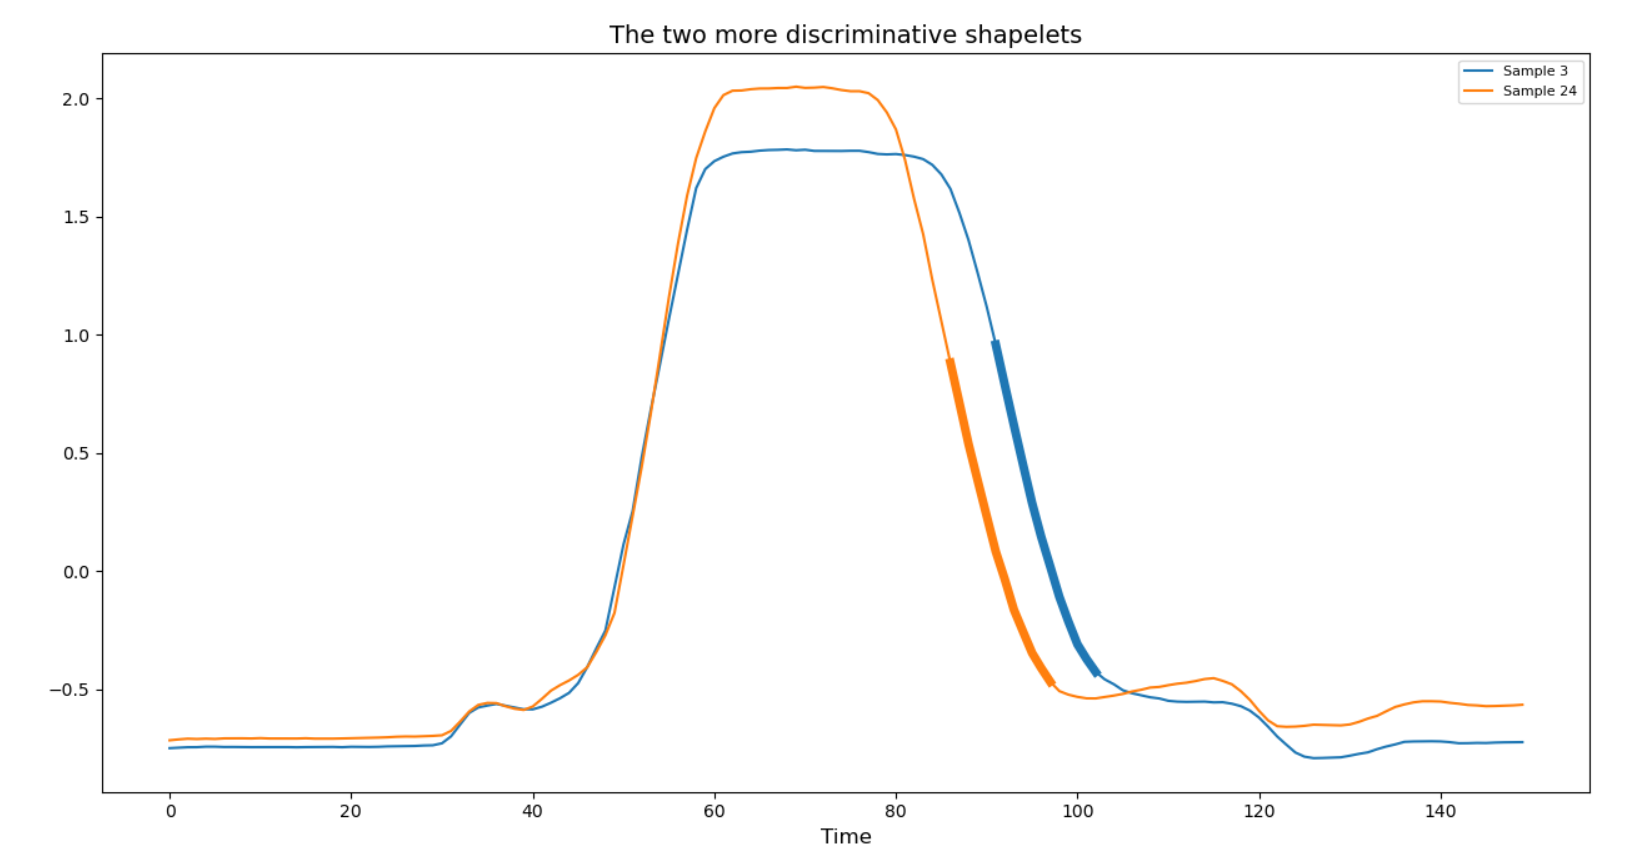
\includegraphics[width=\textwidth]{gfx/Overview of shapelet transform.png}
	\captionsetup{justification=centering}
	\caption{Example of Shapelet Transform.}
	\label{fig:OverviewShapeletTransform}
\end{figure}

\subsubsection*{ROCKET}

ROCKET stands for Random Convolutional Kernel Transform. Using random convolutional kernels, ROCKET is an exceptionally fast and accurate time series classification \cite{dempster_etal_2020}. The Figure \ref{fig:OverviewROCKET} shows an overview of the algorithm. ROCKET takes time series data as input and generates a large number of random convolutional kernels. In simple terms, the kernel is a small matrix that is used for creating a feature map from time series. In ROCKET, all characteristics (e.g. Bias, Length, Weights, Dilation, and Padding) of kernels are random. ROCKET extracts two aggregate features from each feature map produced by each convolutional kernel. The first is the maximum value, and the second is the proportion of positive values (ppv). Maximum value includes the calculation of global max pooling and global average pooling and both are used for dimensionality reduction in convolutional neural networks (CNN). In global average pooling, we take the average of each feature map, and in global maximum pooling, we take the largest value from each feature map. The ppv directly represents the proportion of the input that matches the pattern. The bias term acts as threshold for ppv: the negative bias value means strong matches between the input and the given pattern, and the positive bias value means weak matches between the input and the given pattern. The ppv is the only feature that gives higher classification accuracy. ROCKET produces 2000 (2k) features per time series for 1000 kernels (k) (e.g. max and ppv). The transformed features by ROCKET are used to train any classifier.

\begin{figure}[ht]
	\centering
	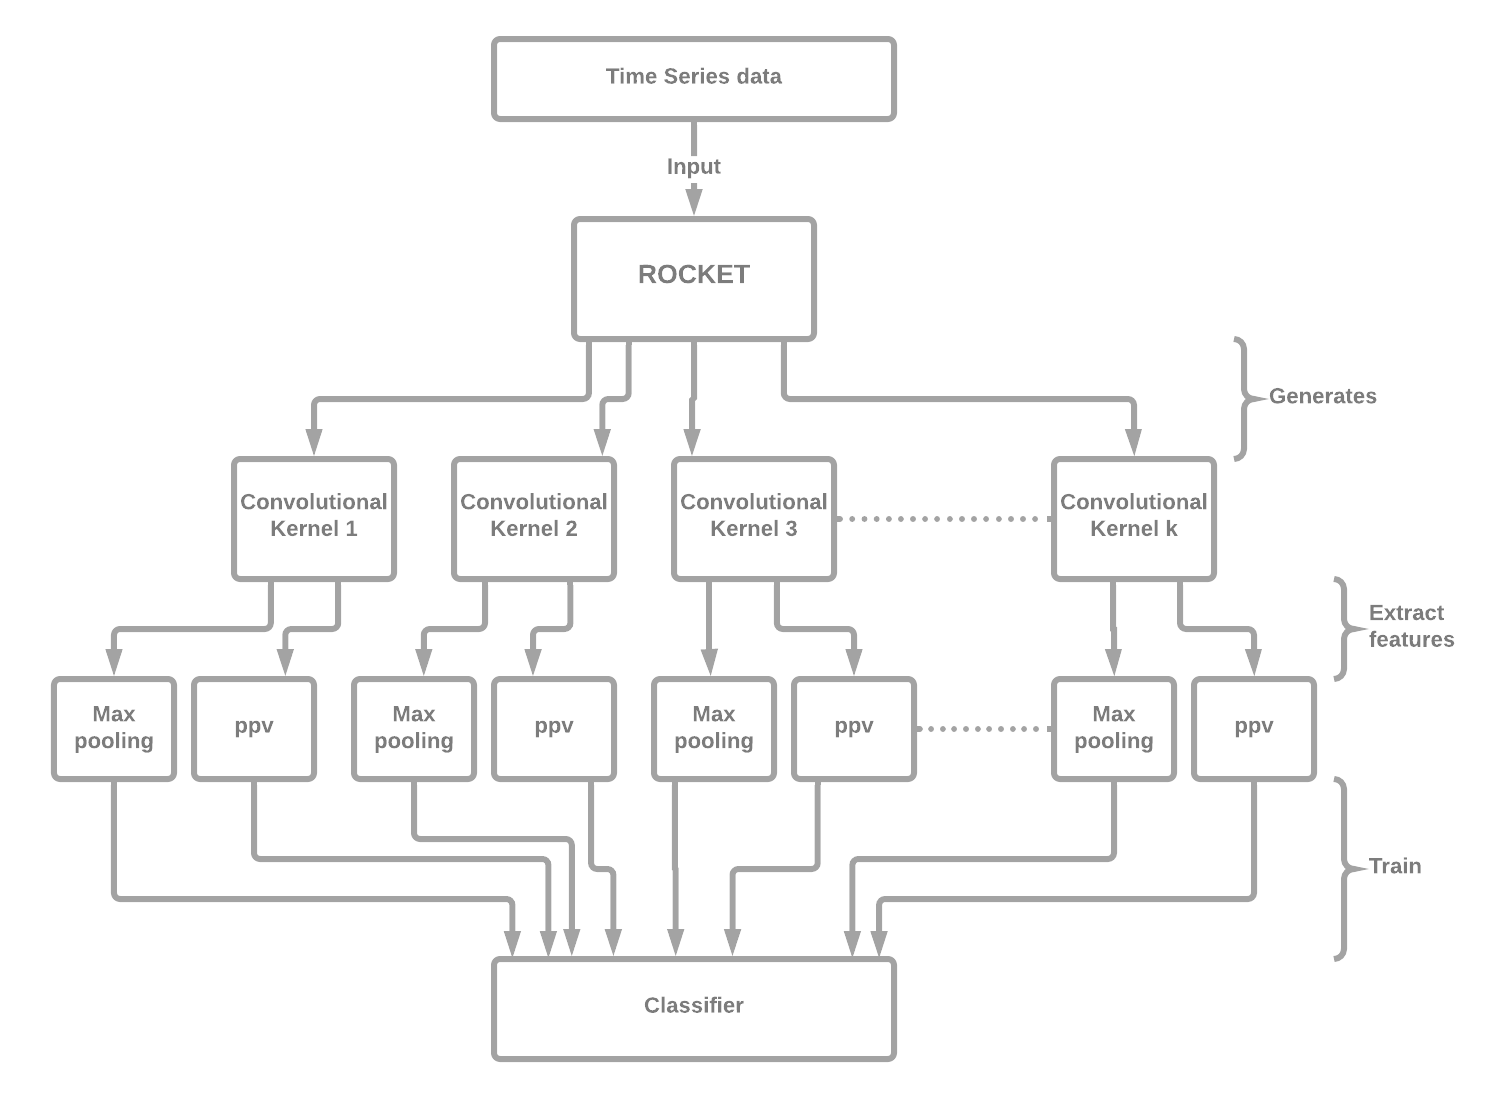
\includegraphics[width=\textwidth]{gfx/Overview of ROCKET.PNG}
	\captionsetup{justification=centering}
	\caption{Overview of ROCKET}
	\label{fig:OverviewROCKET}
\end{figure}

\subsubsection*{RNN Autoencoder}

A Recurrent Neural Network (RNN) is a powerful deep learning (DL) algorithm that works on sequential time series data. Autoencoder (AE) is an unsupervised Artificial Neural Network (ANN) that extracts features from the original data and then reconstructs the data. RNN based AE is an automatic feature extraction method that reduces noise while maintaining important information. Figure \ref{fig:StructureRNNAE} represents the structure of RNN AE consisting of an encoder and a decoder. In the RNN AE training, the input is the original time series data and the output is the reconstructed time series data. In the encoding phase, the input data is efficiently compressed and encoded  then the features are extracted. The extracted features of all frames are fed into the decoder. In the decoding phase, the data is reconstructed back from the reduced encoded representation to a representation that is as close to the original input as possible.

\begin{figure}[ht]
	\centering
	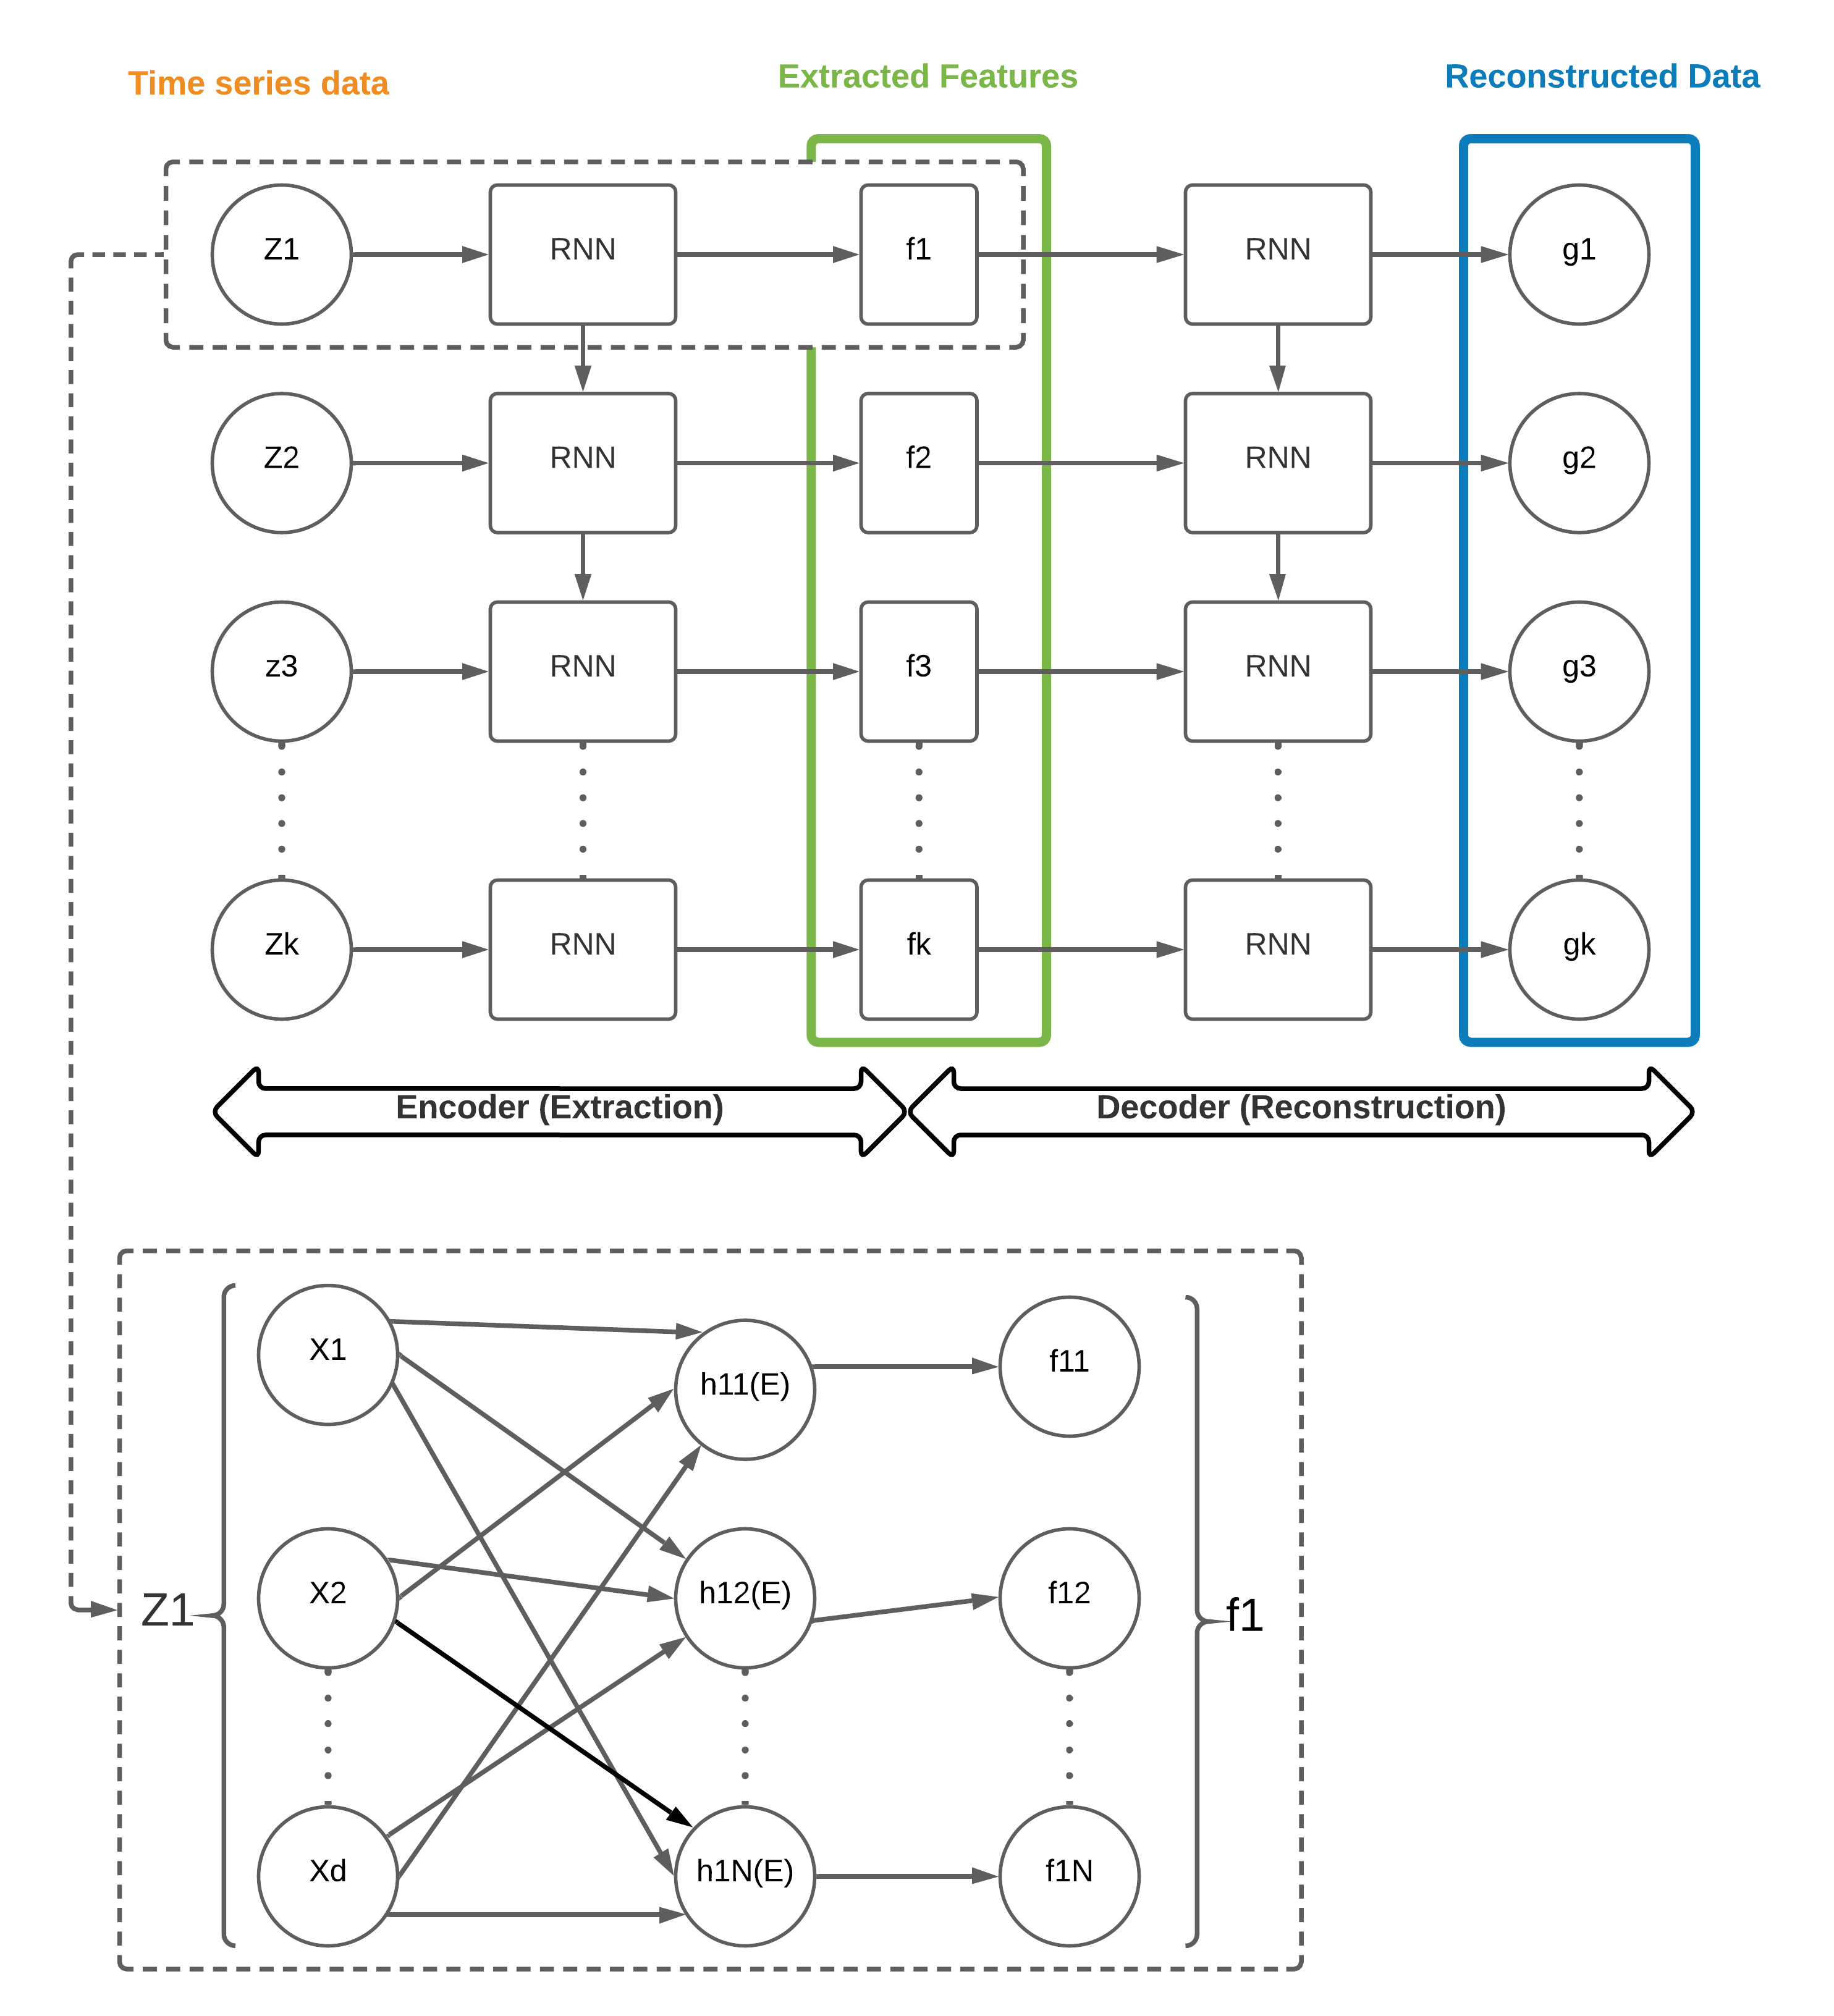
\includegraphics[width=\textwidth]{gfx/Structure of RNN AE.PNG}
	\captionsetup{justification=centering}
	\caption{Structure of the RNN AE}
	\label{fig:StructureRNNAE}
\end{figure}

\subsection{Frequency Domain}
\vspace*{-15mm}
\hfill{\fontfamily{phv}\normalsize\emph{Paul Fährmann}}
\label{sec:feature-extraction:approaches:frequency-domain}
\\\\
The frequency domain of a time series or more specifically of sensor data is a collection of frequencies that represents our sensor data. We transform our sensor data into this frequency domain via the discrete Fourier transform (DFT). We can then use different feature extraction methods to generate features which can be then combined into a real valued vector as defined in Section~\ref{sec:feature-extraction:formal-definition}.
\paragraph{Discrete Fourier Transformation}
To transform the data of sensor $s \in [S]$ of time series $x_{i}\in\mathcal{X}$ with length $l := \tau(i,s)$ into the frequency domain, we use the following function \cite{DBLP:phd/dnb/Kimotho16}:
\begin{equation}
DFT(\omega_k)=\sum\limits_{j=0}^{l-1} v_{i,s}^{(j)} e^{-u\omega_kj},\quad k = 0,\dots,l-1,
\end{equation}
where $\omega_k = \frac{2\pi k}{l}$, $v_{i,s}^{(j)} \in V(s)$ for all $j$, $u$ is the imaginary unit and $DFT(\omega_k)$ is the $k$-th coefficient. For this we can only use sensors with singular values out of a value domain  $V(s)\subseteq\mathbb{C}$.
\subsubsection{Basic Features}
Once the signal is transformed into the frequency domain with $DFT$, basic features like in the time domain can be extracted.\\
Below are a few examples \cite{DBLP:phd/dnb/Kimotho16} of features that can be extracted from the data of one sensor.
\begin{center}
	\begin{tabularx}{.625\textwidth}{ll}
		\hline
		Feature & Formula\\
		\hline
		Maximum Amplitude & $\max(DFT(\omega_k))$\\
		Frequency of Max-Amplitude & $\omega_k|_{max(DFT(\omega_k))}$\\
		Energy of signal & $\sum_{k=0}^{l-1}|DFT(\omega_k)|^2$\\
		\hline
	\end{tabularx}
\end{center}
These features can be extracted from different sensor data and then be put into a singular feature vector as a representation of the whole time series.
\subsubsection{BOSS}
Another way to utilize the frequency domain is BOSS \cite{schafer2015boss} , or Bag of Symbolic Fourier Approximation Symbols.
This method is based on the SFA algorithm and combines it with a bag-of-words approach via quantization using Multiple Coefficient Binning (MCB). Both methods are described below.
\paragraph{Symbolic Fourier Approximation (SFA)}
Transform the time series into the frequency domain using the $DFT$ as described above. Then remove most of the higher frequencies to contain the lowest $c$ coefficients. This is also called low pass filtering. Quantize the real and imaginary parts of the these $c$ Fourier coefficients and put them into words using MCB.
\paragraph{Multiple Coefficient Binning (MCB)}
This technique requires a dataset of time series which can be transformed into the frequency domain. Let's assume we have a data set of size $N \in \mathbb{N_{>0}}$.
As stated above, we take the first $c$ coefficients of each element of a dataset, that results in $N * c$ real and imaginary values. We put these in a $2c \times N$ matrix $A$, such that each row corresponds to the $c$ coefficients of one element of our dataset.
\begin{equation}
A =
\begin{bmatrix}
	\text{Re}_{11} & \text{Im}_{11} & \dots & \text{Re}_{1c} & \text{Im}_{1c} \\
	\vdots & \vdots & \ddots & \vdots & \vdots \\
	\text{Re}_{N1} & \text{Im}_{N1} & \dots & \text{Re}_{Nc} & \text{Im}_{Nc} \\
\end{bmatrix}
\end{equation}
with Re and Im as the real and imaginary values.
We sort the column by value and use equi-depth binning with a prior defined alphabet $\sum$ of size $m\in\mathbb{N_+}$ to create $m$ intervals, which separate the $m$ letters of that alphabet.
\begin{figure}[ht]
	\centering
	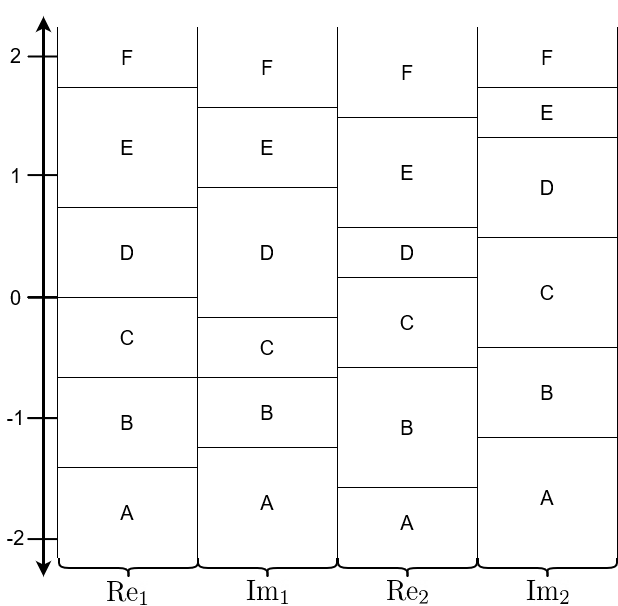
\includegraphics[width=.8\textwidth]{gfx/BOSS_MCB2.PNG}
	\caption{Breakpoints for MCB - example with $m = 6$ and $c = 2$}
	\label{fig:BOSS_MCB}
\end{figure}
In Figure~\ref{fig:BOSS_MCB} we see an example of the MCB with $2$ coefficients, resulting in $2$ real and $2$ imaginary values and an alphabet size of $6$. Transforming a time series into its word using this example we do the following:
\begin{enumerate}
	\item Transform the time series into the frequency domain using $DFT$.
	\item Retain only the first $2$ coefficients, resulting in $4$ values, $2$ real and $2$ imaginary values.
	\item Look in the intervals defined in Figure~\ref{fig:BOSS_MCB} to transform each value into the corresponding letter of the alphabet of size $6$.
	\item Concatenate these letters to one word, representing the time series.
\end{enumerate}
By concatenating the letters to a word we form the word representing the time series. This can be then put into a feature vector for a representation.\\
One question still remains on how to transform the word into the feature representation, defined in Subsection~\ref{sec:feature-extraction:formal-definition}, as this requires a real-valued representation vector.
There are several approaches on how to represent the word in this vector form. We map the letters of the alphabet using $f : \sum \rightarrow \mathbb{R}$ to certain fixed values. Given the intervals for the letters we can take the average value of the interval as a representation of that letter. The mapping $f$ is a bijection; thus we can regain the original word by using the same mapping in reverse.
\subsection{Time and Frequency Domain}
\vspace*{-15mm}
\hfill{\fontfamily{phv}\normalsize\emph{Paul Fährmann}}
\label{sec:feature-extraction:approaches:time-frequency-domain}
\\\\
Using both the time domain and frequency domain of the sensor data of a time series we can extract new types of features that cannot be extracted using just the time or just the frequency domain. We explain two of those approaches.
\subsubsection{Discrete Wavelet Transform (DWT)}
The general motivation for wavelet transforms is, that the frequency domain alone does not provide information on the time in which the frequencies are localized. The wavelet transform tries to solve that by "scanning" over the time series using wavelets of different lengths. When we define the wavelet transform in an abstract way, we arrive at the continuous wavelet transform. We are however interested in the actual application and hence the discrete wavelet transform \cite{DBLP:journals/iet-spr/SangeethaH17}. That is a decomposition of a time series into an amplitude function over two dimensions: time and frequency. This is done using wavelets, which are oscillations with start and end at amplitude value 0. They are used as a sliding filter that is put over the data signal. We need to be able to translate and stretch this filter. In the end, we are able to calculate wavelet coefficients that can be used for a feature vector of the given time series.\\
We need to define when a function or time series $\psi(j)$ is a \textit{wavelet}. $\psi(j)$ is a \textit{wavelet} if the Fourier transformation of $\psi(j)$, named $DFT(\omega_\psi)$ satisfies the following condition:
\begin{equation}
	C_\psi := \int_{0}^{\infty}\frac{|DFT(\omega_\psi)|^2}{|\omega_\psi|} d \omega_\psi < \infty
\end{equation}
This condition describes that the energy of this wave is finite, such that the amplitude will trail off to zero on both sides. 
\begin{figure}[ht]
	\centering
	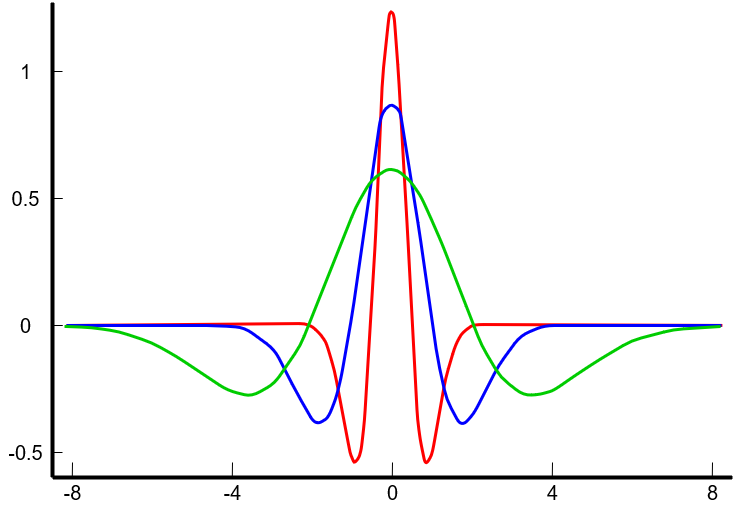
\includegraphics[width=0.5\textwidth]{gfx/DWT_wavelet2.PNG}
	\caption{three examples of wavelet functions.}
	\label{fig:DWT_wavelet}
\end{figure}
Once we have such a wavelet like in Figure \ref{fig:DWT_wavelet}, we can define the discrete wavelet transform as follows:
\begin{equation}
	D[a,b] = \frac{1}{\sqrt{b}}\sum_{j=0}^{l-1} v_{i,s}^{(j)} \psi \left[ \frac{t_{i,s}^{(j)} - a}{b}\right]
\end{equation}
with $l := \tau(i,s)$, $a = k2^{-p}$ and $b = 2^{-p}$.
The parameters $a$ and $b$ stretch and translate the wavelet. Using different values for $a$ and $b$ we scan over the time and over the frequency domain of the original signal. Defining these parameters in the given form where we choose the parameters $k$ and $p$, we assure a dyadic wavelet transformation which has useful properties \cite{DBLP:journals/iet-spr/SangeethaH17}.
Scanning over the original data with different dyadic wavelets we can generate wavelet coefficients which are amplitudes located in time and frequency. These can be viewed as functions that can be analyzed using above mentioned basic time and frequency domain approaches.
\subsubsection{Empirical Mode Decomposition (EMD)}
In the empirical mode decomposition \cite{huang1998empirical} we want to decompose the original time series into intrinsic mode functions (IMF). There is not a lot of mathematical theory behind this method but it transforms the data into a more useful form. 
The idea here is to define a band in which the original data lies. For that an upper \textit{envelope} and a lower \textit{envelope} are defined, such that every value of the original series lies between those envelopes.
For a function to be an IMF, it has to fulfill the two IMF conditions: 
\begin{enumerate}
	\item When counting the  local extrema and the number of crossings through 0, the resulting counts of both must differ by at most 1.
	\item The mean value of the upper and lower envelopes must be equal to zero at every point in the sensor data.
\end{enumerate}

\begin{figure}[ht]
	\centering
	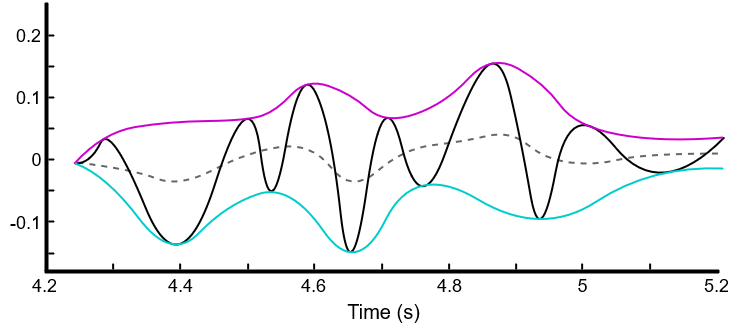
\includegraphics[width=\textwidth]{gfx/EMD_envelopes2.PNG}
	\caption{Example of a time series (black) with upper (magenta) and lower (cyan) envelopes as well as the mean (gray, dashed) of these envelopes.}
	\label{fig:EMD_envelopes}
\end{figure}
These \textit{envelopes} are defined by local minima (lower \textit{envelope}) and local maxima (upper \textit{envelope}) of the original sensor data. To connect these local extrema to a function we use cubic-spline interpolation as seen in Figure~\ref{fig:EMD_envelopes}. Each extrema is connected to the next extrema via a polynomial function of degree 3 \cite{DBLP:journals/computing/Gfrerer82}.  
Once we have generated the envelopes, we can calculate the mean of these \textit{envelopes}. To calculate the IMF components, we need to use the following sifting process.
\paragraph{Sifting process for $v_{i,s} = h_{10}$}:\\
We subtract the mean of the envelopes from the original data to create a new series of values.
\begin{equation}
	 v_{i,s} - m_{10} =: h_{11}
\end{equation}
where $m_{10}$ is the mean of the envelopes on the original data signal and $h_{11}$ is the new series of values for the first step of sifting.
If the conditions for an IMF are not fulfilled, repeat the this sifting step with the new series $h_{11}$ in the place of $v_{j,s}$ to generate $h_{12}$. That means calculating the upper and lower \textit{envelopes} of $h_{11}$ and subtracting the mean $m_{11}$ of these \textit{envelopes} from our series $h_{11}$ creating $h_{12}$.
\begin{equation}
	h_{11} - m_{11} =: h_{12}
\end{equation}
This sifting process step is repeated until $h_{1m_1}$ fulfills the IMF conditions.
\paragraph{IMF components}
The first IMF component can then be defined as $c_1 = h_{1m_1}$.
Repeating this sifting process with $h_{20} := v_{i,s} - c_1$, we generate $c_2$.
Following this procedure, we can calculate $c_1, \dots , c_n$ as the $n$ IMF components.\\
To generate our feature vector we can use the basic features of the time and the frequency domain on these IMF components and put these into one vector representation of the time series $v_{i,s}$.

\subsection{Windowing techniques}
\vspace*{-15mm}
\hfill{\fontfamily{phv}\normalsize\emph{Sanjay Gupta}}\label{sec:feature-extraction:approaches:windowing}
\\\\
In windowing techniques, time series data is partitioned into several windows with specific lengths, from which vector features are 
extracted and fed to a machine learning classifier. One of the widely used windowing techniques is the sliding window technique.

\subsubsection*{Sliding Windows}
The sliding window method is the most widely used approach in the time series classification. In this approach, the time series 
data is divided into fixed-size windows. If there is an intersection between the two adjacent windows, then this technique is 
called an overlapping sliding window and, if not, it is known as a non-overlapping sliding window. The Figure \ref
{fig:SlidingWindows} shows overlapping and non-overlapping techniques for sliding windows. Each window is transformed into a vector 
of features that are mostly time domain, frequency domain, or time \& frequency domain features. This set of features is then used 
to train different classifiers. The number of data points in the window has a significant impact on the performance of the 
model. However, in any case, the size of the window should be selected in such a way that each window contains enough samples to be 
distinguishable from similar movements. Most of the time, window length is selected by trial and error method. The number of sliding 
windows to be used differs for each algorithm of time series classification. While BOSS used a single sliding window to extract 
words, Word Extraction for time Series cLassification (WEASEL) used many sliding windows of different sizes to extract words \cite
{DBLP:conf/cikm/SchaferL17}. The BOP algorithm uses a sliding window to extract subsequences from time series data. Due to a large 
amount of time series data, the performance of the overlapping sliding window increases compared to the non-overlapping sliding 
window.
\begin{figure}[ht]
	\centering
	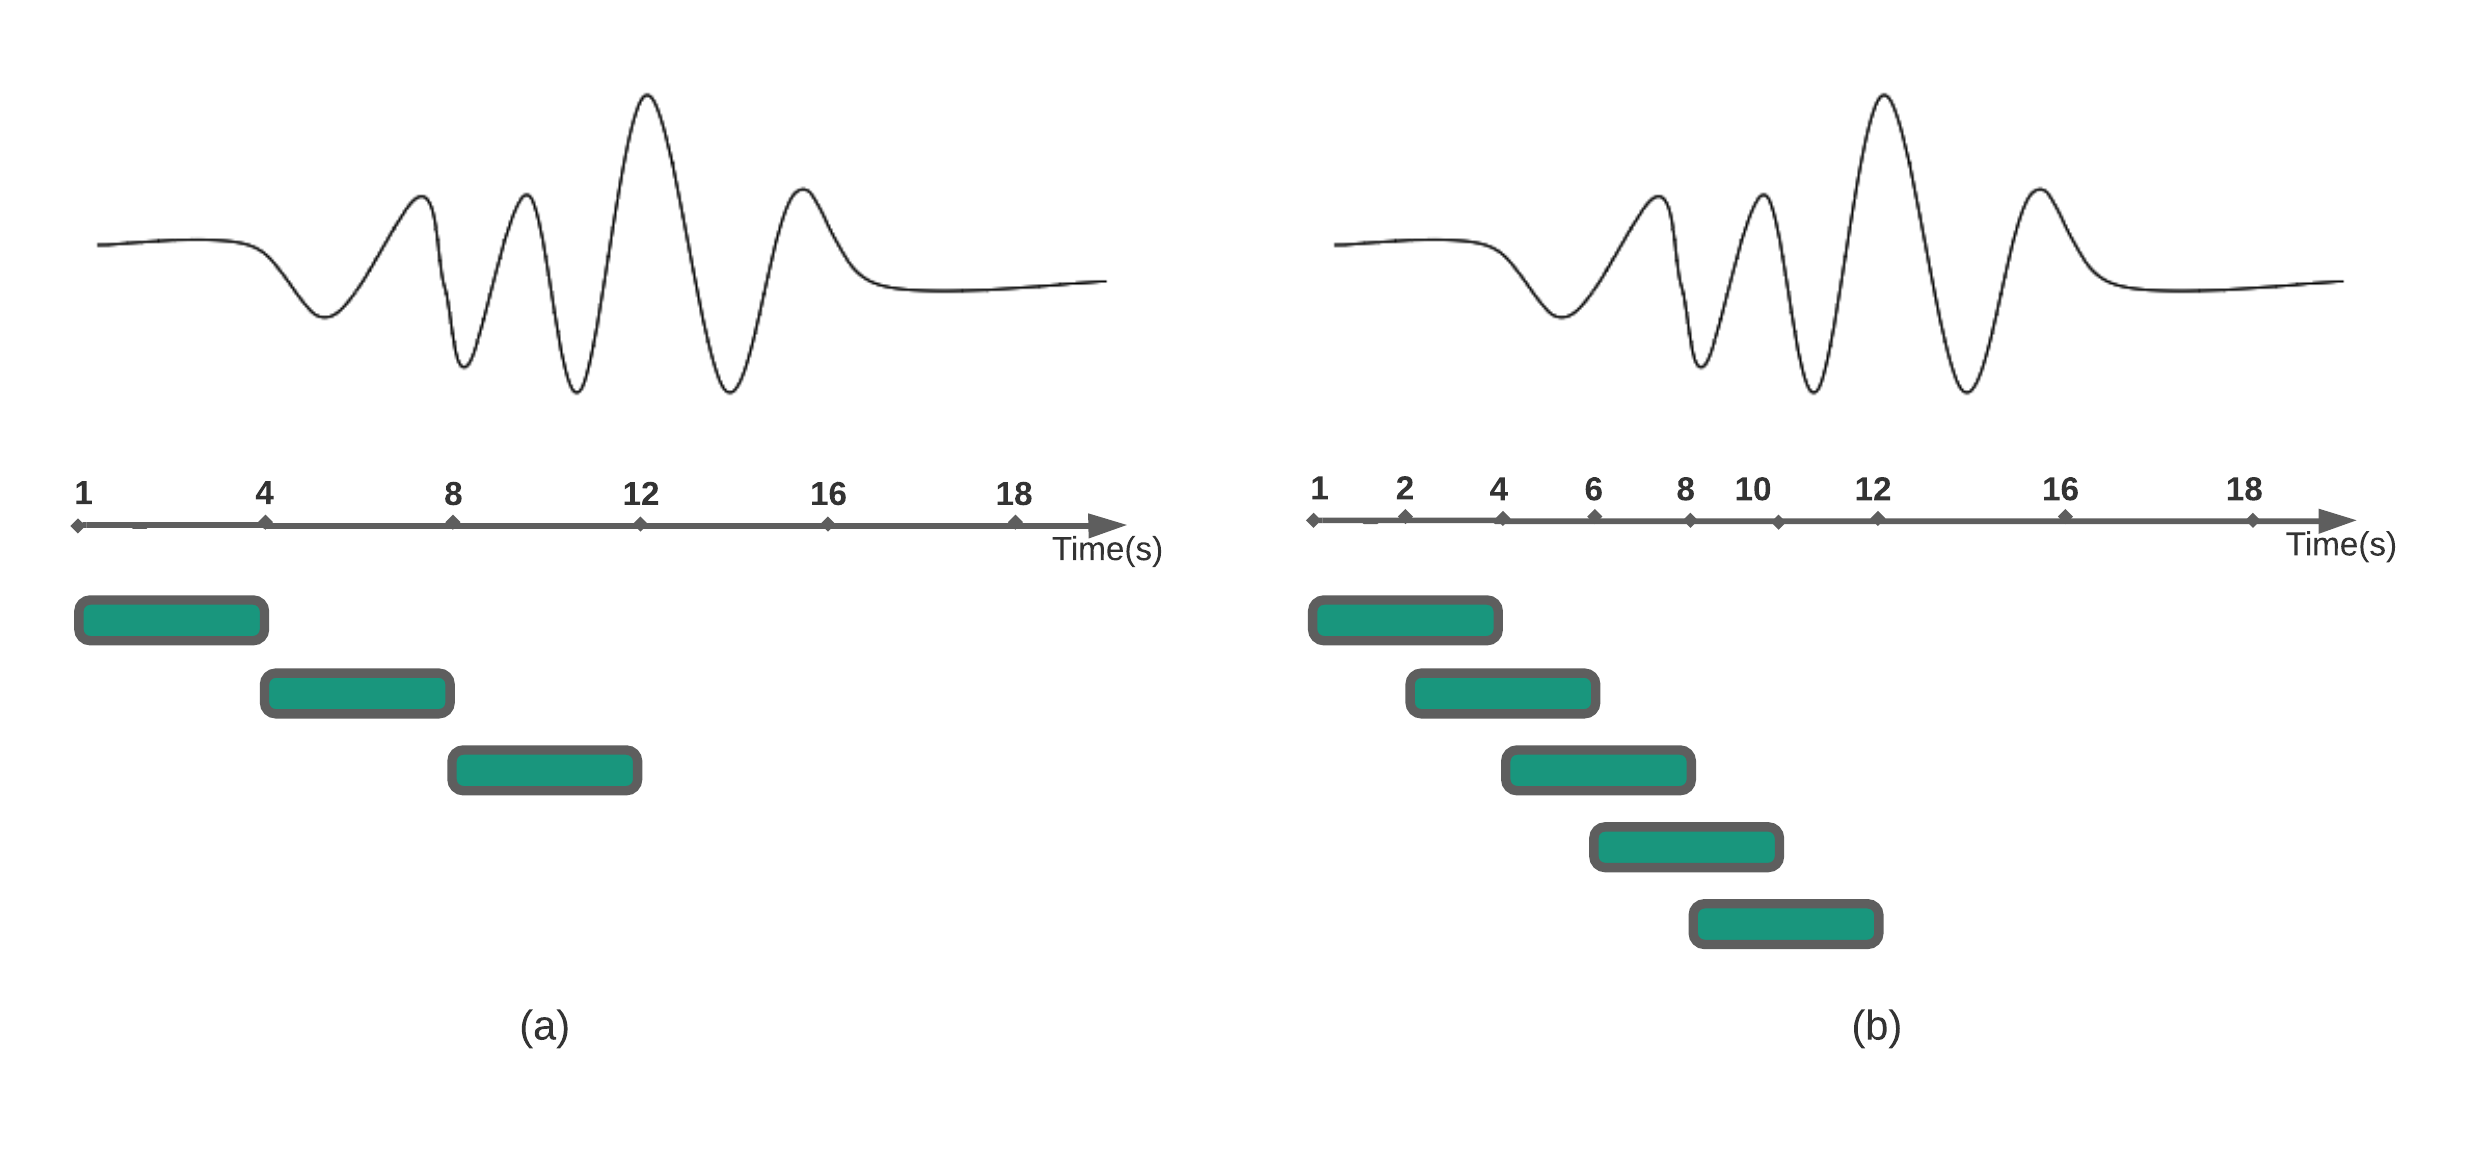
\includegraphics[width=\textwidth]{gfx/Sliding windows.png}
	\captionsetup{justification=centering}
	\caption{4s sliding windows. (a) Non-overlapping; (b) Overlapping-2s sharing.}
	\label{fig:SlidingWindows}
\end{figure}
% Approaches Setion end.

% Evaluation Setup start.
\section{Evaluation Setup}
\vspace*{-15mm}
\hfill{\fontfamily{phv}\normalsize\emph{Paul Fährmann}}
\label{sec:feature-extraction:evaluation-setup}
\\\\
For the evaluation of a feature extraction method, we can look at the feature set or feature vector that this method creates. In order to evaluate a feature vector, we look how well it can be used in various classification or regression problems.\\
In general, we can use the classification and regression models from the following chapters and the loss functions that are used there for our evaluation setup.
In detail that means we control for the entire pipeline except the feature vector and the loss of the model. The loss of the model can then be interpreted as a loss for the feature vector. By swapping different feature vectors in the same setup, the loss for these different feature vectors can be determined. These losses can be compared to each other and so determined what the better and what the worse feature vectors are. It also shows which feature extraction method, on average, performs better on a dataset.
It is important to note though, that the evaluation of a feature extraction method is only meaningful in the specific context or pipeline in which the evaluation was done.
But it can be used for feature selection. The method that extracts the most useful features will get the best evaluation on their extracted feature vectors for this exact pipeline setup. We can then fix the pipeline further by fixing the feature extraction method.\\
A concrete, simple example for this evaluation setup would be a classification problem using the feature vectors of time series of a labeled dataset and the leave-one-out cross validation 
with the $k$-nearest neighbor ($k$-NN) classifier. The evaluation setup would now look as follows:
\begin{enumerate}
	\item Fix the pipeline: fixed model, choose $k$ (e.g. $k = 5$) and the distance metric (e.g. euclidean distance)  for $k$-NN as well as the loss function (e.g. RMSE = root mean square error). Also fix the dataset $\mathcal{X}$.
	\item Transform all $x \in \mathcal{X}$ into their feature vectors via $g_1(x) = z \in \mathbb{R}^d$ with a feature extraction method $g_1$.
	\item Use leave-one-out cross validation with the loss function and the $k$-NN model to calculate the average loss over the entire dataset $\mathcal{X}$.
	\item Repeating step 2 and 3 with $g_2, \dots, g_m$ for $m$ different feature extraction methods. We can compare the average loss for these feature extraction methods and thus evaluate them.
\end{enumerate}
This example demonstrates the evaluation setup for a simple classification scheme. The same setup can be adapted to various different classification and regression schemes. For that we replace parts of this setup. For example, for a regression problem we would replace the model with a regression model and use a loss function for regression problems. Again the leave-one-out cross validation loss over a data set is then used as an evaluation for the used feature vector.
\paragraph{Leave-One-Out Cross Validation}
Given a loss function $l$, a model $M$ and a data set $\mathcal{X}$. The leave-one-out cross validation is given by generating $R := |\mathcal{X}|$ training sets $\mathcal{X}/\{x_i\}$ with $x_i \in \mathcal{X}$ for $i \in [R]$. We train the model $M$ on these data sets, generating fully trained models $M_1, \dots, M_R$. Then we evaluate the classification/regression for the one left out instance, e.g. for $M_1$ we calculate the loss with $l$ for the instance $x_1 \in \mathcal{X}$.
Averaging the loss over all the trained models and evaluated instances, we get the leave-one-out cross validation.

% Evaluation Setup end.

% \section{Related Work Section 2}
% \label{sec:related:sec2}

% \Blindtext[3][2]

% \section{Related Work Section 3}
% \label{sec:related:sec3}

% \Blindtext[4][2]

% \section{Conclusion}
% \label{sec:related:conclusion}

% \Blindtext[2][1]
